\documentclass[11pt]{article}
\usepackage[margin= 1in]{geometry}
% insert a picture
%\begin{Figure}[H]
% \centering
%\includegraphics[scale=2,angle=30][width=0.5\textwidth]{fig1/Treemap2.png}
% %\vspace{-0.1 in}
%  \caption{The Tree map of April 1st shows a less anomalous situation where the magnitudes of different servers may be close. Tree map rectangles with smaller sizes (left) could also be viewed via a zoom and pan interaction with respect to blocks on the right.}
% \label{Fig:treemap2}
% \vspace{-0.1 in}
%\end{figure}

%insert a table
%\begin{table}
%\begin{tabular}{|l|l|l|}
%\hline
%h1&h2&h3\\
%\hline
%a&b&c\\
%\hline
%\end{tabular}
%\end{table}
\usepackage{cite,times,amsmath,algorithm,algorithmic,cases}
\usepackage{graphicx}
\usepackage{grffile}
\usepackage{indentfirst}
\begin{document}
\title{Analysis of Climatological Data}
\author{Xiaoying Yu\\Central Michigan University\\yu3x@cmich.edu
\and Ting Li\\Central Michigan University\\li2t@cmich.edu
\and Hesham Salman\\Central Michigan University\\salma1hh@cmich.com}
\maketitle
\newpage
\begin{abstract}
\end{abstract}
\newpage
\section{Introduction}
Climate is a term for describing the average conditions in a long period. Annual Climatological Summaries offer valuable information to researchers over thousands of reporting in the United States. Much attributes are collected to form the climatical data, such as temperature, precipitation, longitude, latitude, location, location name, and so on. These data stimulates researchers to dig out much useful information to predict the weather changing.

The data set that we discuss is from National Oceannic And Atmospheric Administration(NOAA)\cite{center2010national}. NOAA collects the whole data from daily weather forecasts, severe storm warnings and climate monitoring to fisheries management, coastal restoration and supporting marine commerce\cite{center2010national}.  There are several attributes in the data set, such as station, station name, elvation, latitude, longitude, date, the departure from normal monthly temperature(DPNT), the departure from normal monthly precipitation(DPNP), number days in month with maximum temperature greater than or equal 90 F(DT90), number days in month with maximum temperature less than or equal 32 F(Dx32). This data covers more than 5,000 stations in United Stated, and it records the report data from January in 2014 to November in 2014 of every station.

As for the data set, we hypothesized that elevation had some bearing relationship on the departure from normal temperature or precipitation. Basing on the hypothesis, we take several steps to testify it, for example, cleaning the noisy data, normalizing the data, finding the associational rule of elevation and DPNT, an the associational rule of elevation and DPNP, classifying the data, finding the cluster of the data. To be specific, we also use Java to clean and normalize the big data, which has 62,503 tuples. In the classification, we randomly choose 63\% of the data to build a classifier, and then test the rest data. When referring to this step, we also apply python to converting a comma-separated values(CSV) file to aircraft rescue and firefighting(ARFF) file. In the visualization, we applied Data-Driven Documents JavaScript to visualization the relationship of the association rules. The main tool that we use to find the association rules, classification, and clustering, we apply the weka that is a collection of machine learning algorithms for data mining tasks\cite{hall2009weka}. We concluded several findings. First of all, elevation does have an effect on precipitation: as elevation increase, precipitation tends to normalize. Secondly, when the elevation is normal, most of the monthly DPNT or DPNP tend to be normal.

In the following sections, the first section introduces the data cleaning and normalization. The next section explains how to get the association rules and the visualization of the rules. Then we discuss the classification process basing on five attributes, which are longitude, latitude, DPNT, DPNP, elevation. Furthermore, we also fucus on the clustering to find out the cluster of elevation and DPNT, and the cluster of elevation and DPNP. Finally, we summarized the result that we get from the project.

\section{Related Work}

\section{Data Cleaning and Normalization}
The data we have has nine attributes that were mentioned before, and every month has around 5642 records of different stations. As for the big database, we found there are 262 ``unknown'' value filled in the station, longitude, and latitude value sets, and 12,759 records contain ``-9999'' value in the DPNT or DPNP or both. The total data tuples reach to 62,053. In other words, the percentage of the missing value is $( 262 + 12759 ) / 62053 * 100\% = 22\% $.
\subsection{Data Cleaning}
With the missing data of the first instance, we choose Complete-case method\cite{han2006data}. That is, 262 ``unknown'' tuples are removed. As to the second instance, we refer to the annual document from the NOAA. ``-9999'' was used to represent the missing value in the elevation, DPNT, and DPNP columns. For the correctness, we use Ad Hoc method to record all the ``-9999'' with ``0''. We use this method because DPNT and DPNP are the departure values. ``0'' will not produce big influence on the normalization.
\subsection{Data Normalization}
When we read the data, there is a big difference between the maximum value and the minimum value of these columns(elevation, DPNT, DPNP, longitude, latitude. According to this situation, we applied Z-score normalization method to normalize all these value sets. The Z-score equation is given in Equation \eqref{z-score}.
\begin{equation}
Z-score = \frac{v-\mu}{\delta} \label{z-score}
\end{equation}
where $\mu$ and $\delta$ are the mean and standard deviation of attribute v, respectively.

Specifically, each attribute was calculated in the following steps. First of all, the average of DPNT/DPNP/elevation/longitude/latitude are calculated as $\mu$. Secondly, we apply $|v-\mu|$ to calculate the absolute values of each attribute. Then, we get the average of these absolute values, which is taken as standard derivation $\delta$. Finally, we apply Equation\eqref{z-score} to calculate the Z-score.
After that, we classify five categories of each attribute. For example, elevation has normal, low, very low, high, very high status; DPNT has normal, cold, very cold, warm, very warm. As the normal status in this five attribute, we set the standard derivation of five attributes to the range of (-1, 1). Low or cold are usually set into the normalized range (-2, -1). The very low or very cold status are set the normalized number is less than -2. The same as the high/warm and very high/very warm, which are set into the normalized range (1,2) and greater than 2, respectively.

\section{Clustering}
Clustering the data allowed insights into the distribution of the data points and the identification of different groups. The groups were clustered on two parameters: DPNT, and DPNP. Before clustering, the data set was divided into a training set and a testing set. In order to split the data, the data sets were processed by a Java program which had a 68.3\% chance of selecting each data point for the training set (with replacement). Values had a 32.7\% chance of being selected for the testing set. Only normalized data points were used for the clustering of values. Clustering was carried out with the Simple K Means algorithm, with the intention of finding five clusters for DPNT and DPNP. The reasoning behind five clusters is so that areas can be described as being average, above/below average, far above/below average in temperature and precipitation.

\begin{figure}[h!]
\centering
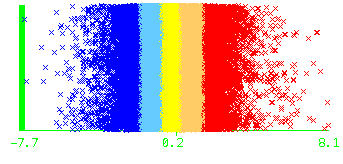
\includegraphics[width=10cm]{dpnt_cluster}
\caption{Clustering of DPNT. From Left to right, the clusters are: Very Cold, Cold, Average, Warm, Very Warm}
\label{fig:dpnt_cluster}
\end{figure}

\begin{figure}[h!]
\centering
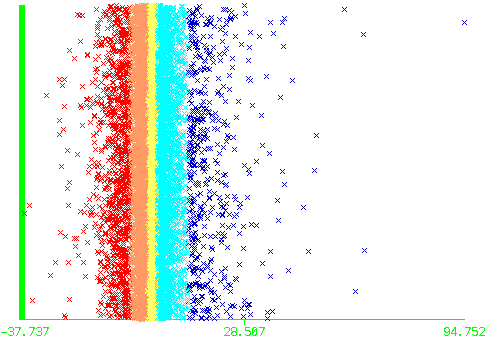
\includegraphics[width=10cm]{dpnp_cluster}
\caption{Clustering of DPNP. From Left to right, the clusters are: Very Dry, Dry, Average, Wet, Very Wet}
\label{fig:dpnp_cluster}
\end{figure}

\begin{figure}[h!]
\centering
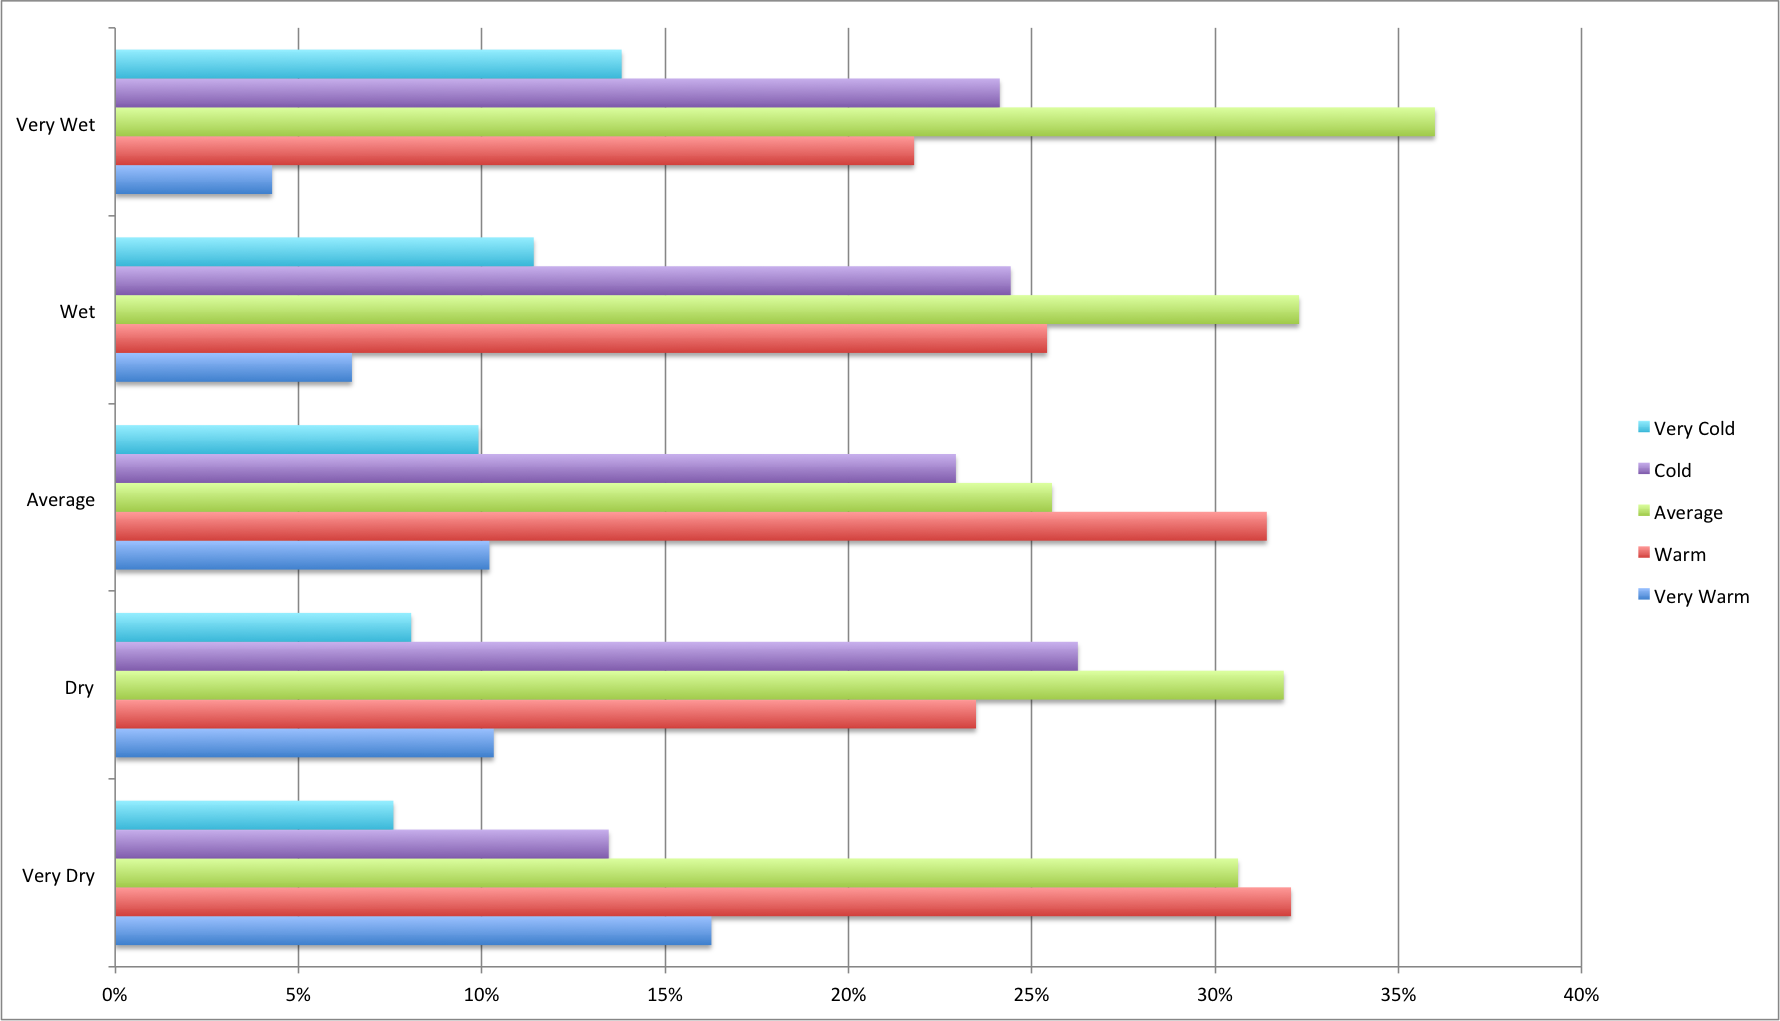
\includegraphics[width=10cm]{ClassDistributions}
\caption{The distributions of precipitation classes within each temperature cluster}
\label{fig:class_distributions}
\end{figure}


The distribution in figure \ref{fig:dpnt_cluster} is such that very warm cluster contains ~10\% of the data (6195 data points), the warm cluster accounts for ~29\% of the data (17756 data points), the average cluster accounts for ~28\% of the data(17235 data points), the cold cluster accounts for ~24\% of the data (14729 data points) and the very cold cluster accounts for ~9\% of the data (5869 data points). The distribution in figure \ref{fig:dpnp_cluster} is such that very dry cluster contains ~2\% of the data (1157 data points), the dry cluster accounts for ~27\% of the data (16785 data points), the average cluster accounts for ~63\% of the data(38992 data points), the wet cluster accounts for ~7\% of the data (4336 data points) and the very wet cluster accounts for ~1\% of the data (1157 data points). 

In general, 2014 tended to be dryer and warmer than previous years. Variations within each group also existed. Areas with less precipitation tended to be warmer, and areas that had more precipitation tended to be colder, as can be seen in figure \ref{fig:class_distributions}. The differences between each of these classes are significant, having passed a chi-square test with a p-value of 0.01. 

\section{Conclusion}
When elevation is low or normal, DPNT tends to be normal. When elevation is normal, DPNP tends to be normal.

\bibliographystyle{plain}
\bibliography{bb}
\end{document}